%
% 4-diffmannig.tex -- Differenzierbare Atlanten und
%                     differenzierbare Mannigkfaltigkeiten
%
% (c) 2024 Prof Dr Andreas Müller
%
\section{Differenzierbare Mannigfaltigkeiten
\label{buch:koordinatne:section:mannigfaltigkeiten}}
\kopfrechts{Differenzierbare Mannigfaltigkeiten}
Ausgangspunkt der bisherigen Überlegungen war die Punktmenge $X$, die
aber vollständig strukturlos war.
Zusätzliche Eigenschaften wie die Definition der Konvergenz oder
die Differenzierbarkeit werden einzig durch die Koordinatensysteme
definiert.
Es wird angenommen, dass $X$ eigentlich ``das Gleiche'' ist wie eine
offene Teilmenge $V$ von $\mathbb{R}^n$.
Es wurde schon bemerkt, dass dies Mengen wie eine Kugeloberfläche oder
die Oberfläche eines Torus von den Betrachtungen ausschliesst, obwohl
sich diese aus Teilstücken zusammensetzen, für die es Koordinatensysteme
gibt.
Solche Mengen heissen differenzierbare Mannigfaltigkeiten und sollen
in diesem Abschnitt definiert werden.

%
% Punktmengentopologie
%
\subsection{Punktmengentopologie}
Die Kugeloberfläche, die Oberfläche eines Torus und viele weitere
Beispiele müssen daher erst in Teilstücke aufgeteilt werden, für
welche sich Koordinatensysteme finden lassen.
Das Definitionsgebiet muss dabei die Eigenschaften haben, die der
Wertebereich eines Koordinatensystems als Teilmenge von $\mathbb{R}^n$
hatte, es muss eine offene Menge sein.
Der Begriff einer offenen Menge ist aber auf einer beliebigen Punktmenge
$X$ nicht a priori definiert.
Das Problem kann mit verschiedenen Ansätzen adressiert werden.

%
% Metrik
%
\subsubsection{Metrik}
Eine {\em Metrik} auf einer Punktmenge  $X$
\index{Metrik}
ist eine Funktion
\[
d
\colon
X\times X \to \mathbb{R}
:
(x,y)\mapsto d(x,y)
\]
mit den Eigenschaften
\begin{enumerate}
\item Positiv: $d(x,y)\ge 0$ für alle $x,y\in X$.
\item Symmetrie: $d(x,y)=d(y,x)$
\item Definit: $d(x,y)=0$ genau dann, wenn $x=y$.
\item Dreiecksungleichung: $d(x,y) \le d(x,z)+d(z,y)$ für alle
$x,y,z\in X$.
\end{enumerate}
Eine Menge $X$ mit einer Metrik heisst ein {\em metrischer Raum}.
\index{metrischer Raum}%
Offene Mengen lassen sich nun genau wie in
Definition~\ref{buch:koordinaten:koordinaten:definition:offenemenge}
definieren.

Sowohl der Begriff der Konvergenz einer Folge gegen einen Grenzwert 
wie auch der Begriff der Stetigkeit einer Abbildung zwischen metrischen
Räumen lässt sich auf eine Metrik übertragen.
Eine Folge $x_n\in X$ in einem metrischen Raum mit der Metrik $X$
konvergiert gegen einen Punkt $x\in X$ wenn es für jedes $\varepsilon>0$
ein $N$ gibt derart, dass $d(x_n,x)<\varepsilon$ ist für $n>N$.
Cauchy-Folgen können analog definiert werden.
Eine Abbildung $f\colon X\to Y$ zwischen metrischen Räumen mit
Metrik $d_X$ bzw.~$d_Y$ ist stetig im Punkt $x_0$, wenn es für jedes
$\varepsilon>0$ ein $\delta > 0$ gibt derart, dass
$d_Y(f(x),f(x_0))<\varepsilon$ für alle Punkte $x\in X$ mit
$d_X(x,x_0)$.

%
% Topologie als Menge von offenen Mengen
%
\subsubsection{Topologie als Menge von offenen Mengen}
Statt die Konstruktion der offenen Mengen auf das vorhandensein einer
Metrik abzustützen, kann man auch die offenen Mengen direkt spezifizieren.

\begin{definition}[Topologie]
\label{buch:koordinaten:koordinaten:definition:topologie}
Sei $X$ eine Punktmenge und $\mathscr{T}$ eine Menge von Teilmengen
von $X$, genannt die {\em offenen Mengen}, mit den folgenden Eigenschaften:
\index{offene Menge}%
\begin{enumerate}
\item Die leere Menge $\emptyset \in \mathscr{T}$ und die ganze Menge
$X\in \mathscr{T}$ sind offen.
\item Für jede Familie $U_i\in \mathscr{T}$ mit $i\in I$ von offenene
Mengen ist die Vereinigung
\[
\bigcup_{i\in I}U_i \in\mathscr{T}
\]
offen.
\item Für jede {\em endliche} Familie $U_i$, $i=1,\dots,m$ von offenen
Mengen ist
\[
\bigcap_{i=1}^m U_i \in\mathscr{T}
\]
offen.
\end{enumerate}
Eine solche Menge von Teilmengen von $X$ heisst eine {\em Topologie}
\index{Topologie}%
auf $X$.
Eine Menge $X$ mit einer Topologie $\mathscr{T}$ heisst ein
{\em topologischer Raum}.
\index{topologischer Raum}%
\end{definition}

Man kann zeigen, dass die durch die 
Definition~\ref{buch:koordinaten:koordinaten:definition:offenemenge}
definierten offenen Mengen auf einem metrischen Raum
die Eigenschaften einer Topologie wie in
Definition~\ref{buch:koordinaten:koordinaten:definition:topologie}
erfüllen.

Der Begriff der Konvergenz einer Folge $x_n\in X$ gegen einen Grenzwert
$x\in X$ kann auf eine Topologie $\mathscr{T}$ übertragen werden.
Die Folge ist konvergent, wenn es für jede offene Menge $U\in\mathscr{T}$
mit $x\in U$ ein $N$ gibt derart, dass $x_n\in U$ für $n>N$.
Auch die Stetigkeit einer Abbildung $f\colon X\to Y$ zwischen topologischen
Räumen kann mit den Topologien $\mathscr{T}_X$ bzw.~$\mathscr{T}_Y$
definiert werden.
Die Abbildung ist stetig im Punkt $x_0$ wenn es für jede offene Menge
$V\in \mathscr{T}_Y$ mit $f(x_0)\in V$ eine offene Menge $U\in \mathscr{T}_X$
gibt derart, dass $f(U)\subset V$.

Es gibt allerdings topologische Räume, die sich nicht mit einer
Metrik definieren lassen.
Für die Zwecke dieses Buches sind sie jedoch nicht relevant.
Wir werden nur topologische Räume betrachten, die mindestens
lokal homöomorph zu offenen Mengen in $\mathbb{R}^n$ sind, deren
Topologie durch die Metrik in $\mathbb{R}^n$ definiert ist.
Wir können daher immer davon ausgehen, dass wir mindestens lokal
eine Metrik zur Verfügung haben, mit der Stetigkeit definiert
werden kann.
Dies bedeutet aber noch nicht, dass wir eine koordinatensystemunabhängige
Längenmessung haben.
Erst die Konstruktion eines metrischen Tensors und der Integration entlang
einer Kurve macht dies möglich und führt auf den Begriff der Riemannschen
Mannigfaltigkeit.
\index{riemannsche Mannigfaltigkeit}%
\index{Mannigfaltigkeit!riemannsch}%

%
% Homöomorphismus
%
\subsubsection{Homöomorphismus}
Seien jetzt $X$ und $Y$ zwei topologische Räume $f\colon X\to Y$ eine
stetige Abbildung.
Ist $f$ umkehrbar und ist $f^{-1}\colon Y\to X$ ebenfalls stetig, dann
lassen sich die beiden topologischen Räume mit den Mitteln der
Punktmengentopologie nicht unterscheiden.
Jede konvergente Folge in $X$ wird von $f$ auf eine konvergente Folge
in $Y$ abgebildet und umgekehrt.
Offene Mengen in $X$ werden in offene Mengen in $Y$ abgebildet und
umgekehrt.

\begin{definition}[homöomorph, Homöomorphismus]
Eine Abbildung $f\colon X\to Y$ zwischen topologischen Räumen heisst ein
Homöomorphismus, wenn sie umkehrbar ist und $f$ wie auch $f^{-1}$
stetig sind.
\index{Homoomorphismus@Homöomorphismus}%
Die beiden topologischen Räume heissen {\em homöomorph}.
\index{homoomorph@homöomorph}%
\end{definition}

Die Koordinatenabbildungen einer stetigen Struktur auf $X$ sind
Homöomorphismen, ebenso die Koordinatenwechsel.

%
% Karten
%
\subsection{Karten}
Eine stetige Struktur verwendet Homöomorphismen, um auf einer Menge $X$
die gleiche topologische Struktur wie in einer offenen Menge in
$\mathbb{R}^n$.
In einem topologischen Raum ist der Begriff der offenen Menge definiert.
Daher kann man versuchen, den Vergleich mit einer offenen Menge von
$\mathbb{R}^n$ für offene Menge von $X$ herzustellen.
Eine Karte von $X$ ist ein Koordinatensystem auf einer offenen Teilmenge
von $X$.

\begin{definition}[Karte]
Eine {\em Karte} von $X$ besteht aus einer offenen Menge $U_\alpha\subset X$
und einer stetigen Abbildung
\[
\varphi_\alpha
\colon
U_\alpha\to V_\alpha\subset\mathbb{R}^n
:
P
\mapsto
(x^1(P),\dots,x^n(P)),
\]
die ausserdem ein Homöomorphismus von $U_\alpha$ auf $V_\alpha$ ist.
Wir schreiben eine Karte auch als Paar $(U_\alpha,\varphi_\alpha)$
\index{Karte}%
\end{definition}

Ein Koordinatensystem $\varphi$ auf der Menge $X$ ist automatisch eine
Karte $(X,\varphi)$.
Eine Karte drückt aus, dass sich der topologische Raum auf dem
Kartengebiet nicht von einer offenen Menge des Raumes $\mathbb{R}^n$
unterscheiden lässt.

%
% Atlanten
%
\subsection{Atlanten und differenzierbare Mannigfaltigkeiten}
%
% fig-karten.tex
%
% (c) 2025 Prof Dr Andreas Müller
%
\begin{figure}
\centering
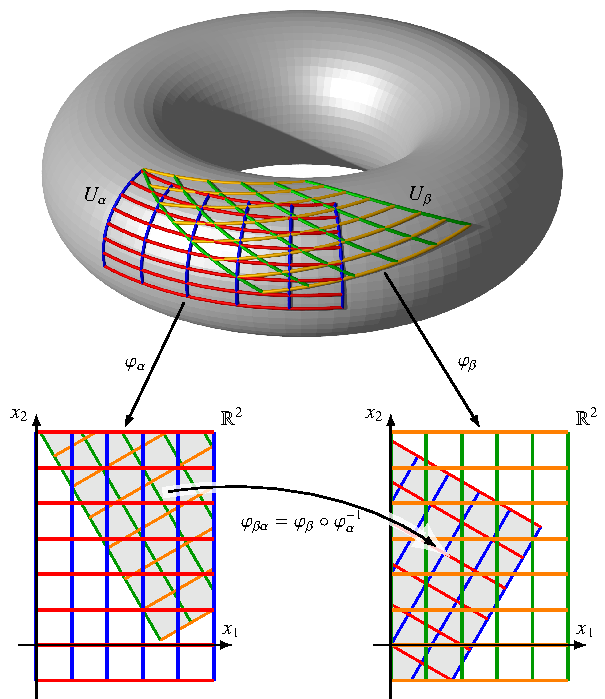
\includegraphics{chapters/020-koordinaten/images/karten.pdf}
\caption{Karten und Kartenwechsel auf einem Torus
\label{buch:koordinaten:fig:toruskarten}}
\end{figure}
%
%
% fig-koordinatenwechsel.tex
%
% (c) 2024 Prof Dr Andreas Müller
%
\begin{figure}
\centering
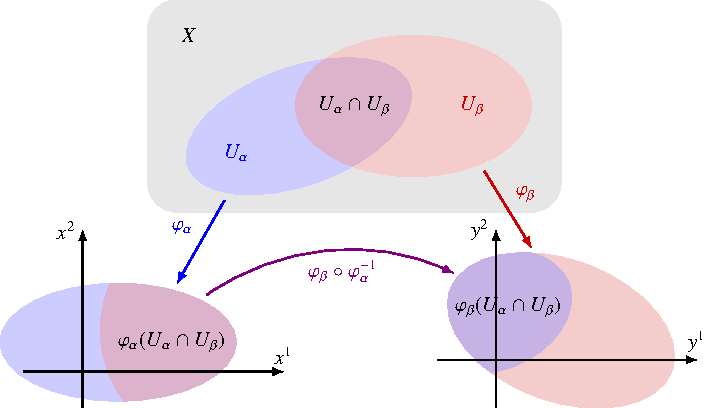
\includegraphics{chapters/020-koordinaten/images/koordinatenwechsel.pdf}
\caption{Koordinatenwechselabbildung $\varphi_\beta\circ\varphi_\alpha^{-1}$
zwischen zwei Karten $(U_\alpha,\varphi_\alpha)$ ({\color{blue}blau}) und
$(U_\beta,\varphi_\beta)$ ({\color{darkred}rot}).
\label{buch:koordinaten:diffmannig:fig:koordinatenwechsel}}
\end{figure}
%
Seien zwei Karten $(U_\alpha,\varphi_\alpha)$ und $(U_\beta,\varphi_\beta)$
gegeben derart, dass $U_\alpha\cap U_\beta$ nicht leer ist.
Auf der offenen Teilmenge $U_\alpha\cap U_\beta$ sind daher durch
die Abbildungen $\varphi_\alpha$ und $\varphi_\beta$ zwei
Koordinatensysteme gegegeben, die wir der Einfachheit halber wieder
mit den gleichen Symbolen bezeichnen\footnote{Genauer wäre, sie als
$\varphi_{\alpha|U_\alpha\cap U_\beta}$ und
$\varphi_{\beta|U_\alpha\cap U_\beta}$ zu bezeichnen, was jedoch
etwas schwerfällig ist.}.
Die Koordinatentransformation ist die Abbildung
\[
\varphi_\beta\circ\varphi_\alpha^{-1}
\colon
\varphi_\alpha(U_\alpha\cap U_\beta)
\to
\varphi_\beta(U_\alpha\cap U_\beta)
:
(x_\beta^1,\dots,x_\beta^n)
\mapsto
(x_\alpha^1,\dots,x_\alpha^n)
\]
(Abbildungen~\ref{buch:koordinaten:fig:toruskarten} und
\ref{buch:koordinaten:diffmannig:fig:koordinatenwechsel}).
Sie heisst der {\em Kartenwechsel} von der Karte $(U_\beta,\varphi_\beta)$
zur Karte $(U_\beta,\varphi_\beta)$.
\index{Kartenwechsel}%

\begin{definition}[Atlas]
Ein {\em Atlas} ist eine Familie $(U_\alpha,\varphi_\alpha)_{\alpha\in I}$
von Karten derart, dass die Kartenwechwechsel
$\varphi_\alpha\circ\varphi_\beta^{-1}$ Homöomorphismen
für alle $\alpha,\beta\in I$ sind, für die
$U_\alpha\cap U_\beta\ne \emptyset$ ist.
\end{definition}

\begin{definition}[differenzierbarer Atlas]
Ein {\em differenzierbarer Atlas} ist ein Atlas, dessen
Kartenwechsel differenzierbar sind.
\end{definition}

Zu einer stetigen Struktur auf $X$ gehört der Atlas $(X,\varphi)$,
wobei $\varphi$ alle Koordinatensysteme der stetigen Struktur druchläuft.
Ist sogar eine differenzierbare Struktur auf der Menge $X$ gegeben,
wie sie in
Definition~\ref{buch:koordinaten:koordinaten:definition:diffbareestruktur}
definiert worden ist, dann bilden die Karten $(X,\varphi)$, wobei
$\varphi$ die Koordinatensysteme der differenzierbaren Struktur
durchläuft, einen differenzierbaren Atlas.

Für die Kugeloberfläche ist es nicht möglich, ein Koordinatensystem
zu finden, welches die ganze Kugeloberfläche abdeckt.
Dieses Phänomen trifft auch bei vielen anderen geometrischen Formen ein.
Ein Atlas ermöglicht, sich bei der Konstruktion auf lokale Betrachtungen
in der Umgegung eines Punktes zu beschränken.

\begin{definition}[differenzierbare Mannigfaltigkeit]
Eine {\em differenzierbare Mannigfaltigkeit} ist eine Menge $X$, die überdeckt
wird von den Definitionsgebieten eines differenzierbaren Atlas auf $X$.
\index{differenzierbare Mannigfaltigkeit}%
\index{Mannigfaltigkeit!differenzierbar}%
\end{definition}

Nach dieser Definition müsste die zweidimensionale Kugeloberfläche eine
differenzierbare Mannigfaltigkeit sein.
Das nachfolgende Beispiel zeigt, wie ein differenzierbarer Atlas
für die Kugeloberfläche gefunden werden kann.

\begin{beispiel}
\label{buch:koordinaten:diffmannig:beispiel:stereographisch}
%
% fig-stereographisch.tex
%
% (c) 2024 Prof Dr Andreas Müller
%
\begin{figure}
\centering
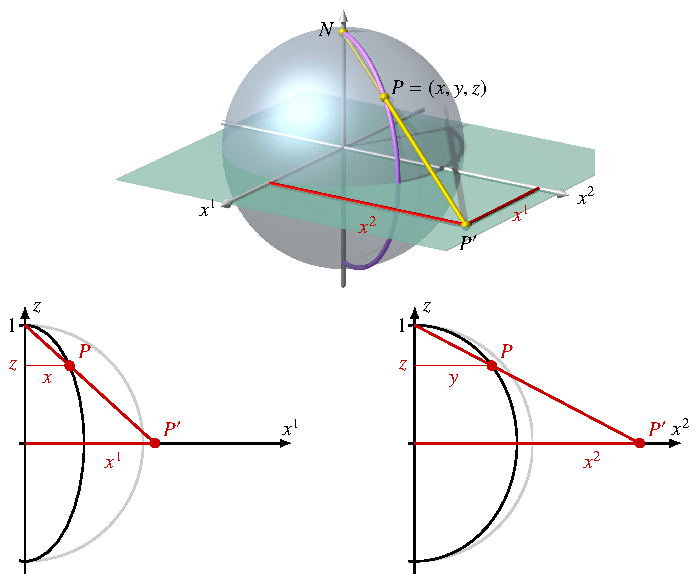
\includegraphics{chapters/020-koordinaten/images/stereographisch.pdf}
\caption{Stereographische Projektion eines Punktes $P$ mit Koordinaten
$(x,y,z)$ auf einer Kugeloberfläche auf die Äquatorebene mit den
Koordinaten $x^1$ und $x^2$.
\label{buch:koordinaten:diffmannig:fig:stereographisch}}
\end{figure}
%
Um zu zeigen, dass die zweidimensionale Kugeloberfläche
\[
S^2
=
\{
(x,y,z)\in\mathbb{R}^3
\mid
x^2 + y^2 + z^2 = 1
\}
\]
eine differenzierbare Mannigfaltigkeit ist, muss ein differenzierbare
Atlas konstruiert werden.
Dazu sind mindestens zwei Karten notwendig.
Wir konstruieren die Karten als stereographische Projektion von den
beiden Polen $N=(0,0,1)$ und $S=(0,0,-1)$ aus.
Als Definitionsbereich der Karten verwenden wir
\[
U_+
=
S^2\setminus \{ (0,0,1)\}
\qquad\text{und}\qquad
U_-
=
S^2\setminus \{ (0,0,-1)\}.
\]
Abbildung~\ref{buch:koordinaten:diffmannig:fig:stereographisch}
gestattet, die Kartenabbildung zu ermitteln.
Der Punkt $P$ mit den Koordinaten $(x,y,z)$ auf der Kugeloberfläche
wird auf den Punkt mit den Koordinaten $(x^1,x^2)$ abgebildet.
Der Strahlensatz besagt, dass
\[
\left.
\begin{aligned}
x : x^1
&=
(1-z) : 1
\\
y : x^2
&=
(1-z) : 1
\end{aligned}
\quad
\right\}
\qquad
\Rightarrow
\qquad
(x^1,x^2) = \frac{1}{1-z}(x,y).
\]
Auf die gleiche Weise kann man auch die stereographische Projektion vom
Südpol aus berechnen.
Als Kartenabbildungen verwenden wir daher
\[
\varphi_+
\colon
(x,y,z)
\mapsto
\frac{1}{1-z}
(x,y)
\qquad\text{und}\qquad
\varphi_-
\colon
(x,y,z)
\mapsto
\frac{1}{1+z}
(x,y).
\]



Die Umkehrabbildungen sind etwas kompliziert auszudrücken, werden
aber auch nicht wirklich benötigt, nur die Zusammensetzung
$\varphi_{\mp}\circ\varphi_{\pm}^{-1}$ müssen berechnet daraufhin
untersucht werden, ob sie differenzierbar sind.
%
% fig-stereowechsel.tex
%
% (c) 2024 Prof Dr Andreas Müller
%
\begin{figure}
\centering
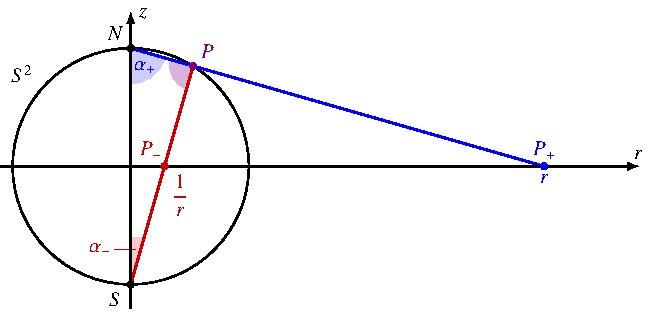
\includegraphics{chapters/020-koordinaten/images/stereowechsel.pdf}
\caption{Die stereographische Projektion $\varphi_+$ vom Nordpol
der Kugel aus bildet den Kugelpunkt $P$ auf den Punkt $P_+$ ab, die 
stereographische Projektion vom Südpol bildet ihn auf $P_-$ ab.
Die Kartenwechselabbildung $\varphi_-\circ\varphi_+^{-1}$ bildet $P_+$
auf $P_-$ ab.
Da $P$ auf dem Thales-Kreis über der Strecke $NS$ liegt, ist der Winkel
bei $P$ ein rechter Winkel und die Winkel $\alpha_+$ und $\alpha_-$
sind komplementär.
Es folgt, dass das Produkt der $r$-Koordinaten der Punkte $1$ ist.
\label{buch:koordinaten:diffmannig:fig:stereowechsel}}
\end{figure}
%
Die ist mit einem viel einfacheren geometrischen Argument möglich,
welches in Abbildung~\ref{buch:koordinaten:diffmannig:fig:stereowechsel}
erklärt wird.
Die Karte $\varphi_+$ bildet $P$ auf $P_+$ ab, $\varphi_-$ bildet
$P$ auf $P_-$ ab.
Da $P$ auf dem Thales-Kreis über der Strecke $NS$ liegt, ist der Winkel
$P$ ein rechter Winkel und die Winkel $\alpha_+$ und $\alpha_-$ sind
komplementär.
Die $r$-Koordinate von $P_-$ ist 
\[
\tan \alpha_-
=
\cot \alpha_+
=
\frac1{\tan\alpha_+}
=
\frac1{r}.
\]
Daraus lässt sich ableiten, dass die Kartenwechselabbildung
\[
\varphi_-\circ\varphi_+^{-1}
\colon
V_+\cap V_- \to V_-\cap V_+
:
(x^1_+,x^2_+)
\mapsto
\frac{1}{(x_+^1)^2 + (x_+^2)^2}(x_+^1,x_+^2)
\]
ist, die ganz offensichtlich differenzierbar ist, solange der 
Nenner nicht verschwindet.
\end{beispiel}

Der Begriff des Atlas erlaubt offenbar, lokale Eigenschaften, also
Eigenschaften, die sich in einer kleinen Umgebung eines Punktes 
feststellen lassen, mit Hilfe eines Koordinatensystems zu analysieren,
welches dafür am besten geeignet ist.
Alle anderen Koordinatensystem werden die Resultate ergeben, die mit
der Kartenwechselabbildung umgerechnet werden können.



